\apendice{Documentación de usuario}

\section{Introducción}

En este apartado hablaremos sobre todo lo necesario para realizar la instalación y la puesta a punto del sistema.

\section{Requisitos de usuarios}

Todos los elementos necesarios para poder ejecutar este proyecto son los siguientes.

\begin{itemize}
	\item Terminal basado en Android con una versión igual a Lollipot 5.0 o superior.
	\item Raspberry Pi con conexión a internet por Wifi o Ethernet. En nuestro caso usaremos la Raspberry Pi 3 Modelo B conectada por Wifi.
	\item Una micro SD de al menos 8 gigabytes (el sistema ocupa más de 4 gigabytes).
	\item Es necesario que el terminal y la Raspberry Pi estén conectados a la misma red de Internet.
\end{itemize}
\section{Instalación}

\subsection{Raspberry Pi}\label{sec:instalacionRaspberry}

Comenzaremos con los pasos necesarios para instalar un nuevo sistema operativo en nuestra Raspberry Pi.\\
El primer paso es conectar nuestra micro SD a un ordenador a través de un adaptador y formatearla como podemos ver en \ref{fig:formateo}

\begin{figure}[h!]
	\centering
	\includegraphics[width=0.4\linewidth]{img/formateo}
	\caption{Formateo en exFAT por ser una SD de gran tamaño.}
	\label{fig:formateo}
\end{figure}
Después descargaremos la imagen del sistema operativo que queremos utilizar en nuestra Raspberry. En este caso usaremos \textit{Raspbian} que es el más común para este dispositivo.\\
Podremos descargar la imagen desde la página oficial de Raspberry \cite{raspberry:raspbian}.\\
Una vez dentro de la página de descargas de Raspberry y tras dirigirnos a la opción de \textit{Raspbian}, tenemos dos opciones.

\begin{itemize}
	\item \textit{Raspbian Stretch with desktop}, que es una imagen con escritorio basado en Debian Stretch.
	\item \textit{Raspbian Stretch Lite}, que es una versión reducida de la anterior en la que no contaremos con escritorio.
\end{itemize}

Para nuestro caso, utilizaremos la primera opción ya que necesitamos un escritorio en el que podamos visualizar el estado de nuestra casa mediante la interfaz. Una vez elegimos el sistema con escritorio se nos descargará un archivo \textit{.zip} que contendrá nuestra imagen del sistema.

Ahora que tenemos nuestra imagen del sistema, necesitamos un programa especial para grabar esa imagen en nuestra micro SD. El programa que yo recomiendo y he usado para la grabación de la imagen se llama \textit{Etcher}. \textit{Etcher} es un programa para la grabación de imágenes en SD, que existe en varias plataformas y además es de software libre. Puede ser descargado desde su página oficial \cite{etcher:url}.

Una vez tenemos la imagen descargada, el programa instalado y la micro SD conectada al ordenador, vamos a grabar el sistema operativo.
Para ello abrimos el programa \textit{Etcher} y seguimos los siguientes pasos:
\begin{enumerate}
	\item Pulsamos sobre \textit{Select image} y mediante el explorador de archivos buscamos la imagen que previamente habíamos descargado.
	\item Pulsamos sobre \textit{Select drive} y marcamos nuestra micro SD.
	\item Finalmente pulsamos sobre \textit{Flash} y comenzará a funcionar.
\end{enumerate}

Antes comenzar a grabar la imagen, el aspecto que debería tener el programa es el siguiente:
\begin{figure}[h!]
	\centering
	\includegraphics[width=0.7\linewidth]{img/etcher}
	\caption{Ventana principal del programa Etcher con la imagen cargada.}
	\label{fig:etcher}
\end{figure}

Tras finalizar la grabación de la imagen en la micro SD, Windows no reconocerá la tarjeta y nos dirá que existe un problema con esa unidad, insistiendo en que debemos formatearla. Esto es debido al formato de archivos que utiliza \textit{Raspbian}, que no es posible ser leído en Windows.\\
Ahora mismo, ya tenemos nuestro sistema operativo preparado para arrancar, asi que solo nos queda insertar la micro SD en la Raspberry Pi y encenderla.

Tras arrancar nuestra Raspberry Pi, deberíamos ver un escritorio como el que se muestra en la imagen \ref{fig:escritorio}.

\begin{figure}[h!]
	\centering
	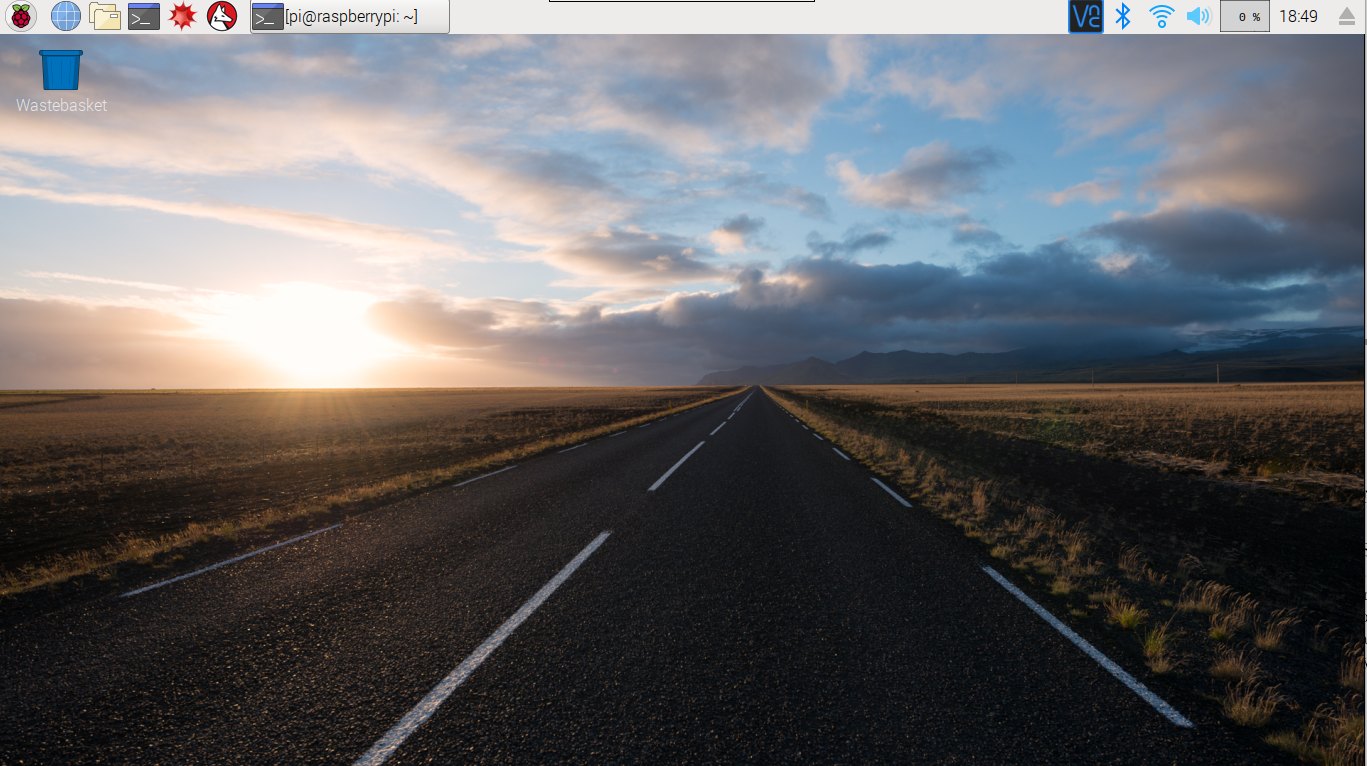
\includegraphics[width=0.8\linewidth]{img/escritorio}
	\caption{Escritorio de Raspbian Stretch en Raspberry Pi.}
	\label{fig:escritorio}
\end{figure}

Lo primero que recomiendo es actualizar el sistema y todos sus paquetes a las versiones más actuales, y activar además las opciones de VNC y SSH desde la configuración de la Raspberry Pi. Una vez hecho todo lo anterior, antes de empezar debemos comprobar que ya venga por defecto preinstalada una versión de Python 3 en nuestro sistema.\\
Para comprobarlo debemos abrir una terminal, ya sea mediante el icono de la barra de tareas o la combinación de teclas Ctrl + Alt + T.\\
Una vez dentro de la terminal, hay que tener en cuenta que el sistema contiene a la vez una versión de Python 2 y una de Python 3. Para diferenciar cuando se utiliza cada una, se sigue la siguiente norma: Siempre que un comando comience por \textit{python}, se usará la versión 2 y cuando el comando comience por \textit{python3} se usará la 3.\\
Teniendo en cuenta esta aclaración, vamos a ejecutar un comando con Python 3 para conocer la versión instalada y a su vez, comprobar que realmente exista una versión de Python 3 instalada. El comando a utilizar es el siguiente: \\ \\
\indent\verb|python3 --version| \\
La salida por pantalla de la terminal debería parecerse a la que se muestra en la imagen \ref{fig:version}.

\begin{figure}[h!]
	\centering
	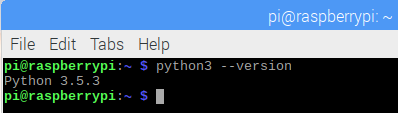
\includegraphics[width=0.8\linewidth]{img/version_python}
	\caption{Salida por pantalla del comando python3 --version.}
	\label{fig:version}
\end{figure}

Sabiendo que nuestro sistema ya tiene una versión preinstalada de Python 3, no tenemos nada más que pasar los archivos \textit{Servidor.py}, \textit{Database.py} y la carpeta \textit{imagenes} a la Raspberrry y ejecutarlos. Podemos pasarlos a través de Internet o simplemente introduciendo una memoria USB en la Raspberry con ellos.
Para que todo quede más ordenado he creado una carpeta llamada \textit{Servidor Raspberry} que contendrá todos los ficheros necesarios. Debería verse como en la imagen \ref{fig:directorio}.

\begin{figure}[h!]
	\centering
	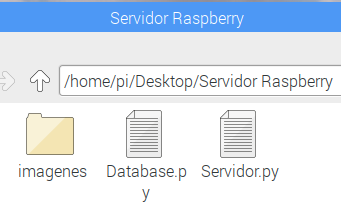
\includegraphics[width=0.8\linewidth]{img/directorio_servidor}
	\caption{Directorio \textit{Servidor Raspberry} que contiene los ficheros especificados.}
	\label{fig:directorio}
\end{figure}

\subsection{Android}\label{sec:instalacionAndroid}

Para comenzar a utilizar la aplicación, lo primero que tenemos que hacer es instalar la apk. Para poder poder instalarla, al ser una aplicación externa que no proviene de ninguna market o tienda, es necesario activar la opción de orígenes desconocidos que permite instalar aplicaciones de terceros. Para activar dicha opción tenemos que seguir los siguientes pasos:

\begin{enumerate}
	\item Entrar en el menú \textit{Ajustes} de nuestro terminal Android.
	\item Dirígete a la opción \textit{Seguridad} dentro de la categoría \textit{Personal}.
	\item Y ahora de nuevo dirígete a la sección \textit{Administración de dispositivos} y la segunda opción \textit{Orígenes desconocidos} es la que debemos activar.
	\item Una vez intentemos activarla, nos mostrará un mensaje de confirmación que deberemos aceptar. 
\end{enumerate}

La apk se puede descargar directamente desde el repositorio del proyecto (\url{https://github.com/MJ0T4/Simulador_Domotica_Raspberry}).

\section{Manual del usuario}

Es esta sección vamos a explicar detalladamente como conseguir ejecutar la parte de \textit{Raspberry Pi} y la parte de \textit{Android} conjuntamente.

\subsection{Raspberry Pi}\label{sec:ejecuciónRaspberry}

Para comenzar con la parte del servidor, he optado por introducir la IP sobre la que se creará el servidor de forma gráfica para que sea más fácil para el usuario. Lo primero es saber como ejecutar el servidor y para ello vamos a seguir los siguientes pasos:

\begin{enumerate}
	\item Abrimos una terminal desde el icono de la barra de tareas o con la combinación de teclas Ctrl + Alt + T.
	\item Necesitamos dirigirnos al \textit{Escritorio} que es donde habíamos guardado previamente los ficheros. Para ello escribimos: \\ \\
	\verb|cd Desktop/|
	\item Ahora que ya nos encontramos en el \textit{Escritorio} debemos ir a la carpeta que donde tengamos los ficheros, en mi caso \textit{Servidor Raspberry}.\\ \\
	\verb|cd Servidor\ Raspberry/|
	\item Por seguridad comprobaremos que realmente los ficheros están ahí mediante el comando \verb|ls|.
	\item Una vez hemos comprobado que tenemos los ficheros \textit{Servidor.py}, \textit{Database.py} y el directorio \textit{imagenes}, ya podemos ejecutar el servidor. Para ello utilizamos el siguiente comando:\\\\
	\verb|python3 Servidor.py|
\end{enumerate}

En la imagen \ref{fig:terminal} se puede observar una terminal con los comandos que hemos mencionado antes.

\begin{figure}[h!]
	\centering
	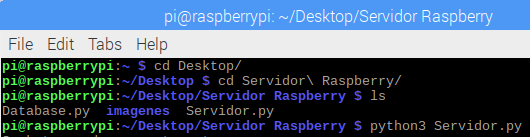
\includegraphics[width=0.9\linewidth]{img/terminal}
	\caption{Terminal con los comandos necesarios para ejecutar el servidor.}
	\label{fig:terminal}
\end{figure}

Después del último comando se abrirá una nueva ventana que será la interfaz que nos mostrará los elementos de nuestra casa que iremos creando y modificando mediante la aplicación de Android. \\
Por defecto, si la aplicación acaba de ser arrancada por primera vez, nos mostrará un error diciéndonos que no ha sido posible montar el servidor sobre esa ip. El error será igual al de la imagen \ref{fig:error}.

\begin{figure}[h!]
	\centering
	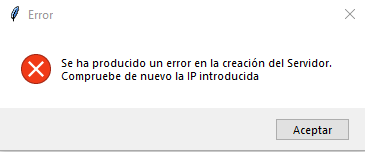
\includegraphics[width=0.8\linewidth]{img/error}
	\caption{Error en la creación del servidor esa una IP.}
	\label{fig:error}
\end{figure}

Cuando pulsemos el botón \textit{Aceptar}, se abrirá una ventana emergente en la que podremos escribir nuestra IP y que será almacenada en la base datos. Por tanto, una vez que hemos introducido nuestra IP correctamente, el resto de veces que carguemos el servidor de nuevo utilizará esta IP. \\
La ventana emergente se verá como la imagen \ref{fig:ventanaEmergente}.

\begin{figure}[h!]
	\centering
	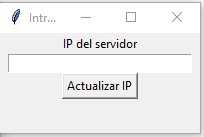
\includegraphics[width=0.4\linewidth]{img/ventanaEmergente}
	\caption{Error en la creación del servidor esa una IP.}
	\label{fig:ventanaEmergente}
\end{figure}

Una vez introducida la IP y pulsado el botón \textit{Actualizar IP}, la ventana se cerrará y se intentará crear de nuevo el servidor. Si la IP introducida es incorrecta, volverá a mostrarse el error y de nuevo la ventana emergente. Si la IP es correcta, el servidor se creará y no saltarán más errores. Si por alguna razón debiésemos reiniciar el servidor, no será necesario introducir de nuevo la IP porque ha sido guardada en la base de datos.\\
Si quisiéramos introducir una nueva IP válida, solo tendríamos que borrar la base de datos manualmente o con la opción existente en la App móvil. \\

\subsection{Android}\label{sec:manualAndroid}

Con la aplicación ya instalada, vamos a hablar sobre las posibilidades que nos ofrece la App y sus ventanas.

\subsubsection{Ventana Principal}

\begin{figure}[h!]
	\centering
	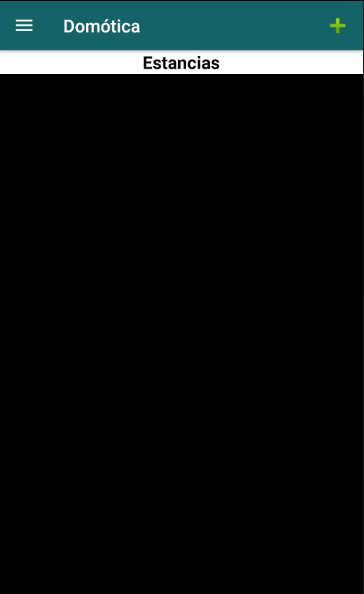
\includegraphics[width=0.35\linewidth]{img/ventanaPrincipal}
	\caption{Ventana inicial y principal de esta aplicación.}
	\label{fig:ventanaPrincipal}
\end{figure}

Cuando se abre la aplicación nos encontramos con la ventana que se muestra en la imagen \ref{fig:ventanaPrincipal}. En ella se mostrarán nuestras estancias, es decir, las diferentes salas de estar que podemos crear. Las salas que podemos crear son \textit{\textbf{Habitaciones}}, \textit{\textbf{Salones}}, \textit{\textbf{Cocinas}} y \textit{\textbf{Baños}}, y cada una de ellas tiene una imagen asignada. \\
En la parte superior, contamos con un menú desplegable que podemos mostrar pulsando sobre las tres líneas blancas horizontales, el título y un botón desde el que podemos desplegar opciones.\\
Pinchando sobre el botón con icono verde y símbolo \textbf{+} se mostrará una ventana emergente con diferentes opciones. En dicha ventana \ref{fig:opcionesEstancias}, tendremos la opción de crear cualquier tipo de las cuatro estancias pulsando sobre su nombre y además elegir un nombre para ella. \\

\begin{figure}[h!]
	\centering
	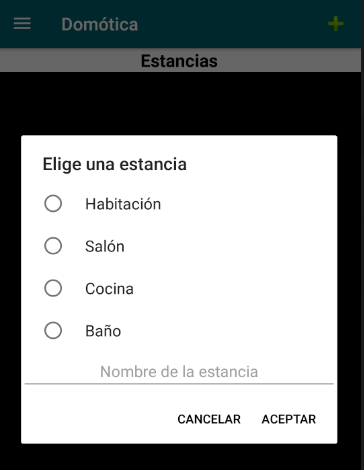
\includegraphics[width=0.4\linewidth]{img/opcionesEstancias}
	\caption{Ventana emergente para la creación de nuevas estancias.}
	\label{fig:opcionesEstancias}
\end{figure}

Tras seleccionar una de las opciones y escribir un nombre para ella, pulsamos sobre el botón \textit{Aceptar} y se creará. Para realizar un ejemplo, crearemos una \textit{Habitación} con el nombre \textit{Habitación}, que podremos ver en la imagen \ref{fig:creacionHabitacion}. \\

\begin{figure}[h!]
	\centering
	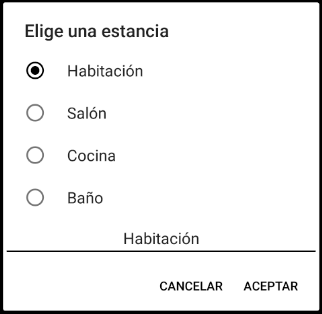
\includegraphics[width=0.5\linewidth]{img/creacionHabitacion}
	\caption{Creación de una nueva \textit{Habitación} mediante la ventana emergente.}
	\label{fig:creacionHabitacion}
\end{figure}

Una vez pulsado el botón \textit{Aceptar} se nos creará la habitación y la ventana principal se nos quedará de la siguiente manera \ref{fig:ventanaPrincipalHabitacion}.\\
Con está habitación ya creada, contamos con las opciones de eliminarla o cambiar su nombre.

\begin{figure}[h!]
	\centering
	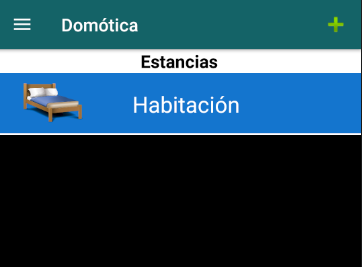
\includegraphics[width=0.5\linewidth]{img/ventanaPrincipalHabitacion}
	\caption{Creación de una nueva \textit{Habitación} mediante la ventana emergente.}
	\label{fig:ventanaPrincipalHabitacion}
\end{figure}

Para poder borrar o cambiar el nombre de la \textit{Habitación} creada anteriormente debemos acceder a su menú contextual. Este menú aparecerá tras pulsar poco más de un segundo sobre ella. Se puede ver en la imagen \ref{fig:menuContextual}.

\begin{figure}[h!]
	\centering
	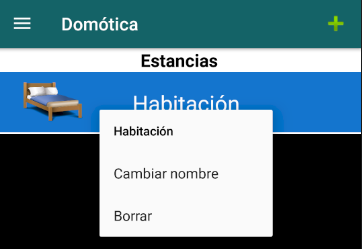
\includegraphics[width=0.6\linewidth]{img/menuContextual}
	\caption{Menú contextual de una estancia}
	\label{fig:menuContextual}
\end{figure}

Si pulsamos sobre la opción \textit{Cambiar nombre} se mostrará una nueva ventana emergente en la que debemos insertar el nombre y pulsar el botón \textit{Aceptar}. Dicha ventana emergente se verá como la imagen \ref{fig:cambiarNombre}

\begin{figure}[h!]
	\centering
	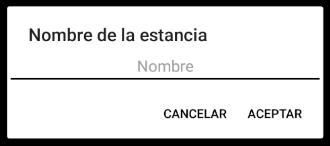
\includegraphics[width=0.6\linewidth]{img/cambiarNombre}
	\caption{Opción \textit{Cambiar nombre} del menú contextual de una \textit{Habitación}.}
	\label{fig:cambiarNombre}
\end{figure}

En cambio, si pulsamos sobre la opción \textit{Borrar} se mostrará un mensaje emergente de confirmación para la realización de dicha acción. El mensaje sería igual al de la imagen \ref{fig:borrar}.

\begin{figure}[h!]
	\centering
	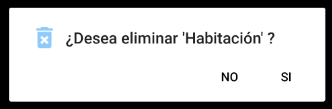
\includegraphics[width=0.6\linewidth]{img/borrar}
	\caption{Opción \textit{Borrar} del menú contextual de una \textit{Habitación}.}
	\label{fig:borrar}
\end{figure}

Para poder realizar todas las acciones a anteriores es necesario estar conectado al servidor, sino se nos mostrará una ventana emergente \ref{fig:ventanaEmergenteError} con un botón que nos dirigirá a la ventana del Servidor. 

\begin{figure}[h!]
	\centering
	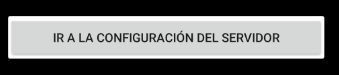
\includegraphics[width=0.6\linewidth]{img/ventanaEmergenteError}
	\caption{Ventana emergente en caso de no estar conectado al servidor.}
	\label{fig:ventanaEmergenteError}
\end{figure}

Si pulsamos sobre las tres líneas blancas horizontales en la barra superior, se desplegará un menú. En este menú tenemos dos opciones:

\begin{itemize}
	\item \textbf{Servidor}, que nos redirigirá a la misma ventana que el botón de la imagen \ref{fig:ventanaEmergenteError}.
	\item \textbf{Borrar base de datos}, que borrará tanto los datos locales como los del servidor.
\end{itemize}

El menú desplegable podemos verlo en la imagen \ref{fig:menuPrincipal}.

\begin{figure}[h!]
	\centering
	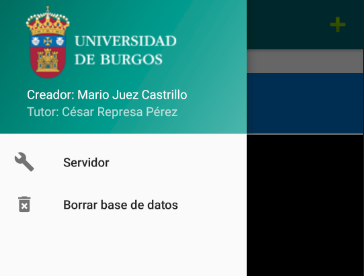
\includegraphics[width=0.6\linewidth]{img/menuPrincipal}
	\caption{Menú principal que se mostrará al pulsar en las tres líneas blancas horizontales}
	\label{fig:menuPrincipal}
\end{figure}

\subsubsection{Ventana Servidor}

Esta es otra de las ventanas de la aplicación desde la que podemos acceder mediante el menú desplegable que se encuentra en la ventana principal(\ref{fig:menuPrincipal}) o mediante el botón de la ventana emergente que se nos muestra cuando queremos realizar una acción y no estamos conectados al servidor (\ref{fig:ventanaEmergenteError}).\\

En la ventana servidor (\ref{fig:servidor}) nos encontramos con dos campos para rellenar:

\begin{figure}[h!]
	\centering
	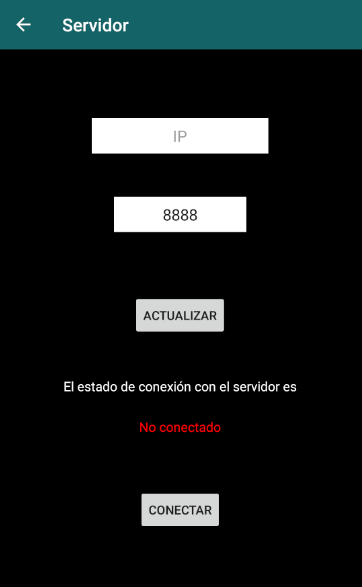
\includegraphics[width=0.6\linewidth]{img/servidor}
	\caption{Ventana \textit{Servidor} de la aplicación.}
	\label{fig:servidor}
\end{figure}

\begin{itemize}
	\item \textbf{IP}, este campo viene vacío por defecto y en él debemos escribir la \textit{IP} del servidor al que queremos conectarnos.
	\item \textbf{Puerto}, este campo viene por defecto como \textbf{8888} y es el puerto que se usará para realizar la conexión, aunque permite la posibilidad de ser cambiado.
\end{itemize}

Una vez hemos escrito la \textbf{IP} y el \textbf{Puerto} al que deseamos conectarnos, solo debemos presionar el botón \textit{Actualizar}. Cuando el botón es pulsado, estos datos son guardados en la base de datos para futuras conexiones, de manera que solo deberíamos realizar este paso una vez. \\
Tras actualizar los datos, ya podemos conectarnos al servidor, así que pulsamos sobre el botón \textit{Conectar} que se encuentra en la inferior. Si la conexión se ha realizado con éxito, nuestra ventana del Servidor se debería ver como la imagen \ref{fig:conectado}, sino se seguiría viendo como la imagen \ref{fig:servidor}.

\begin{figure}[h!]
	\centering
	\includegraphics[width=0.6\linewidth]{img/conectado}
	\caption{Conexión exitosa con el servidor.}
	\label{fig:conectado}
\end{figure}

Esta acción de conectarse al servidor solo deberá realizarse una vez, ya que por defecto en la ventana principal \ref{fig:ventanaPrincipal} tratará de conectarse al servidor con la \textbf{IP} que hayamos guardado en la base de datos desde la ventana del Servidor \ref{fig:servidor}.

Una vez estamos conectados y deseamos volver a la ventana principal, solo debemos pulsar sobre la flecha que se encuentra en la parte superior izquierda de la ventana. De nuevo en ventana principal, vamos a hablar sobre la última ventana.

\subsubsection{Ventana iluminación}

La ventana de iluminación es una ventana desde la cuál podemos crear, modificar y eliminar \textit{Bombillas} para las estancias creadas en la ventana principal. Para acceder a ella, solo debemos encontrarnos en la ventana principal y pulsar sobre la estancia que queremos. Tras esto, nos dirigirá a una nueva ventana como la de la imagen \ref{fig:ventanaIluminacion}

\begin{figure}[h!]
	\centering
	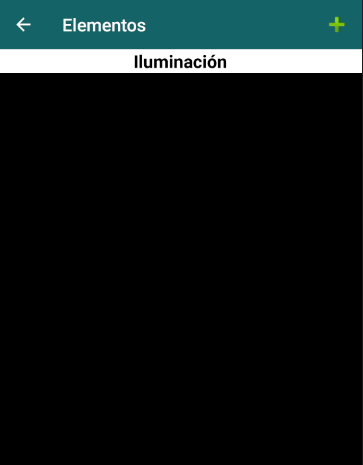
\includegraphics[width=0.6\linewidth]{img/ventanaIluminacion}
	\caption{Ventana iluminación.}
	\label{fig:ventanaIluminacion}
\end{figure}

Pinchando sobre el botón con icono verde y símbolo \textbf{+} que se encuentra en la parte superior derecha, se mostrará una ventana emergente \ref{fig:ventanaEmergenteBombilla} para la creación de bombillas. 

\begin{figure}[h!]
	\centering
	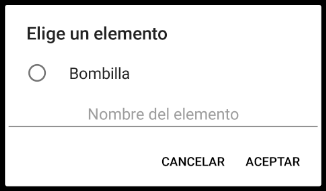
\includegraphics[width=0.6\linewidth]{img/ventanaEmergenteBombilla}
	\caption{Ventana emergente para la creación de una bombilla.}
	\label{fig:ventanaEmergenteBombilla}
\end{figure}

Debemos pinchar sobre la única opción posible, especificar un nombre para ella y pulsar sobre el botón \textit{Aceptar}. Tras hacerlo, se nos creará una nueva \textit{Bombilla} y nuestra ventana de iluminación se verá como la de la imagen \ref{fig:ventanaIluminacion2}.

\begin{figure}[h!]
	\centering
	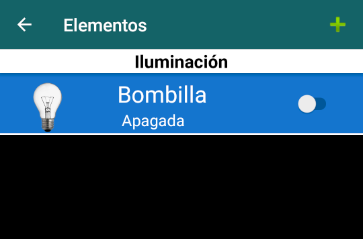
\includegraphics[width=0.6\linewidth]{img/ventanaIluminacion2}
	\caption{Ventana iluminación tras crear una \textit{Bombilla}.}
	\label{fig:ventanaIluminacion2}
\end{figure}

En esta nueva \textit{Bombilla} contamos con una imagen, que nos muestra su estado, su nombre, un texto que también que nos indica su estado y un interruptor para encenderla y apagarla. Para cambiar su estado, es tan sencillo como pulsar el interruptor y ver como se ilumina la bombilla, tanto aquí como en la parte de Python. La imagen \ref{fig:bombillaIluminada} muestra como sería el resultado de pulsar el interruptor.

\begin{figure}[h!]
	\centering
	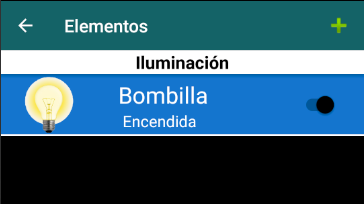
\includegraphics[width=0.6\linewidth]{img/bombillaIluminada}
	\caption{Ventana iluminación con una \textit{Bombilla} encendida.}
	\label{fig:bombillaIluminada}
\end{figure}

Además de todo esto, cada \textit{Bombilla} que creemos, contará con su propio menú contextual \ref{fig:menuContextualBombilla} con las mismas opciones que las estancias (\textit{Cambiar nombre} y \textit{Borrar})  y que se mostrará de la misma manera.

\begin{figure}[h!]
	\centering
	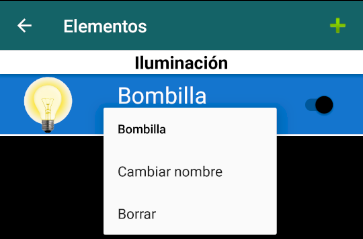
\includegraphics[width=0.6\linewidth]{img/menuContextualBombilla}
	\caption{Menú contextual de una \textit{Bombilla}.}
	\label{fig:menuContextualBombilla}
\end{figure}